\section{The interface Schur-complement system}
\label{sec:sigma-solver}

The last remaining piece for generating our preconditioner is the design of the approximation $\Sigma^\dagger$ and the application of its effective numerical
solution which is hosted exclusively on the CPU. As previously stated, our objective is to arrive at an algorithm that is sublinear in complexity relative to the
size of the overall boundary and yields a good approximation to the exact matrix
$\Sigma=A_{\Gamma\Gamma}-\sum_{i=1}^kA_{\Gamma i}A_{ii}^\varA{-1}A_{i \Gamma}$.
\changed
{The approximations incurred in $\Sigma^\dagger$ are twofold: (a) instead of solving $\Sigma x_\Gamma=b_\Gamma$ exactly, we will substitute a number of V-cycles of an
  appropriately designed multigrid scheme, and (b) we modestly modify the matrix used in this multigrid scheme, using adaptivity, to reduce the cost of direct algebra.}
{We will solve the approximate system $\Sigma^\dagger x_\Gamma=b_\Gamma$ using a multigrid method, which will avoid forming the dense matrix $\Sigma^\dagger$
explicitly. Furthermore, we will leverage adaptive coarsening of the subdomains to reduce the dimensionality of the direct algebra involved in our manipulations.}

\begin{figure}[t!]
\begin{center}
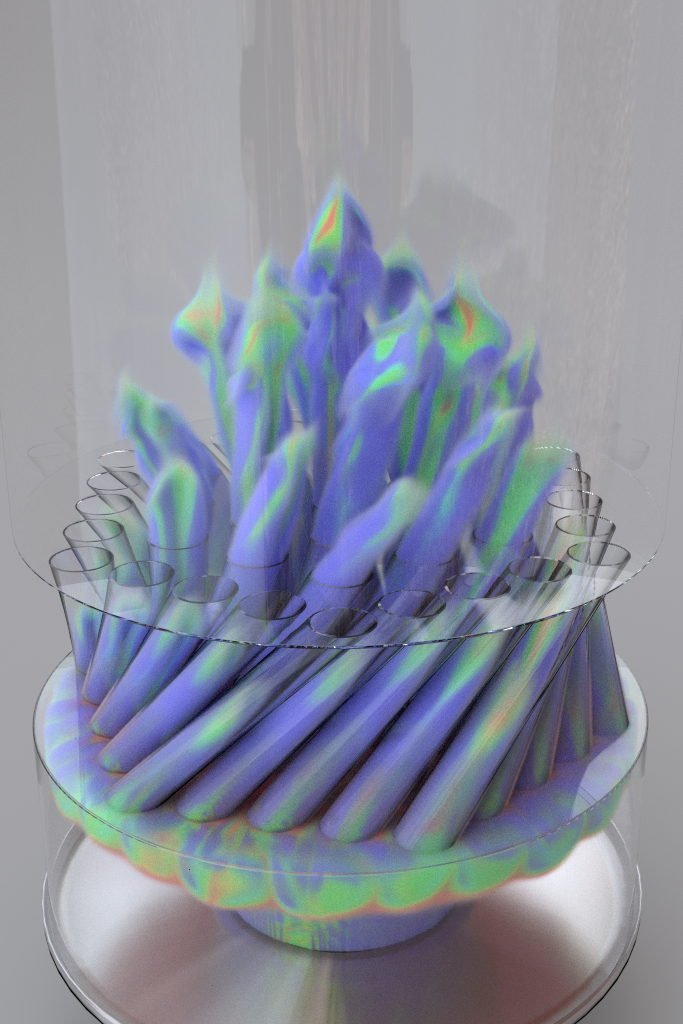
\includegraphics[width=.49\columnwidth]{images/DD/sieve_smoke_150_alternate.png} 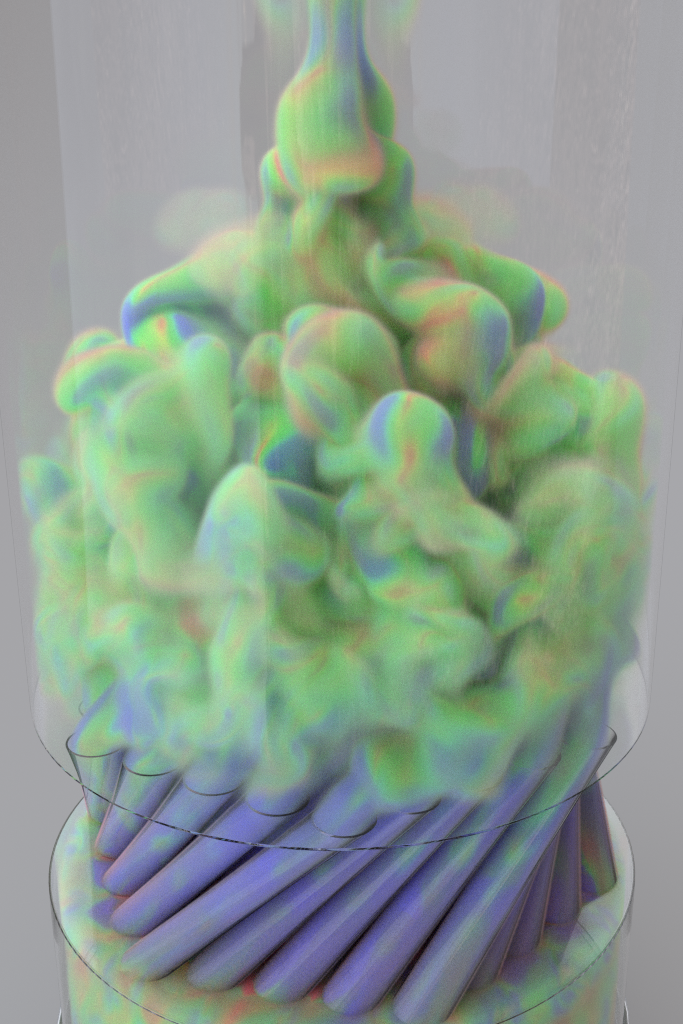
\includegraphics[width=.49\columnwidth]{images/DD/sieve_smoke_255_alternate.png}
\end{center}
\caption{Smoke injected from the bottom of a cylinder, and forced through a
  twisted bundle of cylindrical holes. Color corresponds to vorticity magnitude. Total 1.2B active cells, in a $1024^2\!\times\!2048$ grid.}
\label{fig:sieve}
\end{figure}


\subsection{Multigrid solver for the interface}
\label{sec:interface-multigrid-solver}

The Schur complement matrix $\Sigma$ is not only symmetric and positive definite, but it can further be shown that it is an \emph{elliptic} operator, as it is a
discretization of the continuous and elliptic \emph{Steklov-Poincar\'{e} operator} for the Poisson equation~[\cite{Smith:1996:DDP:238150}]. This suggests that a
multigrid solver (on the interface variables; separate from the multigrid cycles used to approximate the subdomain inverses) could be applicable.
%For such a multigrid scheme, we need a hierarchy of discretizations, a smoother, and appropriate transfer operations.
 The simplest technique for building the multigrid
hierarchy is to use Galerkin coarsening to construct the operator at each
resolution level. However, we do not pursue this option as it requires explicitly computing
the matrix $\Sigma$ at the finest level, which is a computationally expensive proposition. We propose a different conceptual construction of the operator hierarchy,
and design a smoother that can use them indirectly without assembling their explicit matrix form.


We construct the coarser level operators in the following fashion,
$\Sigma^{2h}=A_{\Gamma\Gamma}^{2h}-\sum_{i=1}^kA_{\Gamma
i}^{2h}(A_{ii}^{2h})^\varA{-1}A_{i \Gamma}^{2h}$, where the entire matrix
$A^{h}$ has first been coarsened down to $A^{2h}$ using trilinear interpolation, and
then the individual building blocks are harvested and reassembled for computing
$\Sigma^{2h}$.  While this may appear a plausible choice for the multigrid
hierarchy, and indeed our experiments show that this gives good convergence, the
intuition behind it comes from the following
observation. Suppose we constructed a multigrid hierarchy for the full problem $Ax=b$,
where the right hand side $b$ has non-zero entries \emph{only} on
the interface $\Gamma$, i.e., we are solving the following equation via
multigrid:
\begin{eqnarray}
\label{eqn:sigma-multigrid-intuition}
\begin{bmatrix}
A_{11} & & A_{1\Gamma} \\
& A_{22} & A_{2\Gamma} \\
A_{\Gamma 1} & A_{\Gamma 2} & A_{\Gamma\Gamma}
\end{bmatrix}
\begin{bmatrix}
x_1 \\
x_2 \\
x_\Gamma
\end{bmatrix}
=
\begin{bmatrix}
0 \\
0 \\
b_\Gamma
\end{bmatrix}
\end{eqnarray}

then the solution can be shown to satisfy $x_\Gamma=\Sigma^\varA{-1}b_\Gamma$. Let us further assume that our smoother routine was designed such that it completely
eliminated any residual of equations interior to the subdomains, leaving nonzero residuals only on interface degrees of freedom. We can then interpret our proposed
multigrid procedure, which operates solely on the interface, as algebraically
equivalent to a full-domain multigrid scheme used with a right hand side that is zero
anywhere outside the boundary, as in equation (\ref{eqn:sigma-multigrid-intuition}), combined with a smoother that annihilates residuals on
subdomain interiors.

The terms $\sum_{i=1}^k A_{\Gamma i}A_{ii}^\varA{-1}A_{i \Gamma}$ in the formula of $\Sigma$ correspond directly to this concept of subdomain-interior equations
being solved exactly, and used to eliminate those degrees of freedom from the dimensionality of $\Sigma$. A smoother that can operate on $\Sigma$ directly,
implicitly ensures that all equations in the interior of each subdomain are satisfied at all times. Finally, the restriction and prolongation operators for the
interface-based multigrid solver can be inferred from the transfer operators of the global problem. Note that, for the purposes of this section we depart from the
cell-centered perspective of grid values, as employed for example in the hierarchy construction by \cite{mcadams2010parallel},
and switch to viewing unknowns as stored in the nodes of the \emph{dual} of the typical MAC grid used for the Navier-Stokes discretization (i.e. pressure values
stored on \emph{nodes} of this new grid). We then coarsen the cells in the typical 8-to-1 fashion, using trilinear interpolation. This ensures that interface degrees
of freedom remain fully aligned across levels of the multigrid hierarchy, and that trilinear prolongation of a finer level's interface variables will only need
coarse interface variables as input. Although restriction \emph{into} coarse interface values technically touches interior values as well, the residuals of all such
interior equations will be zero (since the Schur complement operator assumes those equations fully satisfied). Thus the transfer operators we ultimately use in our
cycle are \emph{bilinear interpolation} along the aligned 2D interface surfaces at each level of the hierarchy.


\subsection{Smoothing the Schur-complement system}
\label{sec:schur-complement-smoother}

As previously shown, $\Sigma$ is a symmetric and positive definite matrix. Thus, in principle, damped Jacobi or Gauss-Seidel would have been convergent
smoothers. However, since we do not have access to the explicit matrix form of $\Sigma$, operations that would be required (for example, the diagonal elements of
$\Sigma$) are not readily available. Thus, we take a different approach of designing a smoother that can be iterated without an explicit construction of the matrix.
Using the definition of $\Sigma$, the system $\Sigma x_\Gamma=b_\Gamma$ can be rewritten as:
\begin{eqnarray}
\label{eqn:sigma-smoother-raw}
A_{\Gamma\Gamma}x_\Gamma=b_\Gamma+\sum_{i=1}^k A_{\Gamma i}A_{ii}^\varA{-1}A_{i \Gamma}x_\Gamma
\end{eqnarray}
We can use equation (\ref{eqn:sigma-smoother-raw}) to design a fixed-point
iteration as follows:
\begin{eqnarray}
\label{eqn:sigma-smoother-iteration}
A_{\Gamma\Gamma}x_\Gamma^{(n+1)}=b_\Gamma+\sum_{i=1}^k A_{\Gamma i}A_{ii}^\varA{-1}A_{i \Gamma}x_\Gamma^{(n)}
\end{eqnarray}
One may recognize the similarity of equation (\ref{eqn:sigma-smoother-iteration}) with the analogous matrix form $Dx_\Gamma^{(n+1)}\!\!=b_\Gamma+(L+U)x_\Gamma^{(n)}$
of the Jacobi iteration based on the decomposition $\Sigma=D\!-\!L\!-\!U$, should that have been explicitly available.
Instead of isolating just the diagonal part of $\Sigma$, our decomposition employs the entire 
$A_{\Gamma\Gamma}$ term. In the next section we provide a proof that this iterative scheme will always converge.

The iterative scheme in equation (\ref{eqn:sigma-smoother-iteration}) requires two basic blocks. First, given an already computed right hand side, solving for
$x_\Gamma$ requires solving a sparse symmetric and positive definite system. Since the matrix $A_{\Gamma\Gamma}$ is very sparse and structured, we use a sparse
Cholesky factorization using the Intel MKL PARDISO library, which we have found to be very well-performing especially due to the fact that the interface is
highly structured and admits a very effective nested bisection for reordering its degrees of freedom to maximize sparsity. Second, the right hand side requires the
inverse operator $A_{ii}^\varA{-1}$ for each subdomain. Again, our approach would be to use a Cholesky factorization of $A_{ii}$ (with appropriate reordering)
to solve the inversion problem using forward/backward substitution. Pseudocode for the smoother routine is given below:

\begin{algorithm}
\caption{Application of smoother routine. Input: $b_\Gamma,x_\Gamma^{(n)}$}
\label{alg:interface-smoother}
\begin{algorithmic}[1]
\FOR{$i=1\ldots k$}
\STATE Compute $y_i\leftarrow A_{i \Gamma}x_\Gamma^{(t)}$\COMMENT{sparse; fast}
\STATE Solve $z_i\leftarrow A_{ii}^\varA{-1} y_i$\COMMENT{PARDISO}
\STATE Compute $w_\Gamma^{(i)}\leftarrow A_{\Gamma i}z_i$\COMMENT{sparse; fast}
\ENDFOR
\STATE Compute $f_\Gamma=b_\Gamma+w_\Gamma^{(1)}+\ldots+w_\Gamma^{(k)}$
\STATE Solve $x_\Gamma^{(n+1)}\leftarrow A_{\Gamma\Gamma}^\varA{-1} f_\Gamma$\COMMENT{PARDISO}
\end{algorithmic}
\end{algorithm}

The matrix $A_{\Gamma\Gamma}$ in step 7 has $O(N^{2/3})$ nonzero entries, and we observed that with appropriate reordering (using PARDISO) the nonzero entries in the
Cholesky factors remain asymptotically well below $O(N)$. The subdomain matrices $A_{ii}$, however (step 3) contain on the aggregate $O(N)$ nonzero
entries, which will yield a strictly superlinear number of nonzero entries in their Cholesky factors, even with excellent reordering. We thus proceed to make one
last approximation, in the interest of reducing the dimensionality of these factors, as explained in the following section.

\subsection{Proof of convergence of the interface smoother}

Consider the fixed-point iteration
\begin{equation}
\label{eqn:jacobi-iteration}
\begin{array}{c}
A_{\Gamma\Gamma}\boldsymbol{x_\Gamma}^{(n+1)}=\boldsymbol{b_\Gamma}+\sum_{i=1}^k A_{\Gamma i}A_{ii}^\varA{-1}A_{i \Gamma}\boldsymbol{x_\Gamma}^{(n)} \vspace*{.05in}\\
\Rightarrow S_1\boldsymbol{x_\Gamma}^{(n+1)}=\boldsymbol{b_\Gamma}+S_2\boldsymbol{x_\Gamma}^{(n)}
\end{array}
\end{equation}
where $S_1=A_{\Gamma\Gamma}$ and $S_2=\sum_{i=1}^k A_{\Gamma i}A_{ii}^\varA{-1}A_{i \Gamma}$. Let $\boldsymbol{x_\star}$ be the exact solution
of this iterative scheme, i.e., $\boldsymbol{x_\star}$ satisfies the
equation
\begin{equation}
\label{eqn:jacobi-iteration-exact-solution}
S_1\boldsymbol{x_\star}=\boldsymbol{b_\Gamma}+S_2\boldsymbol{x_\star}
\end{equation}
Subtracting equation (\ref{eqn:jacobi-iteration-exact-solution}) from equation
(\ref{eqn:jacobi-iteration}) gives
$$
\label{eqn:jacobi-iteration-error}
S_1\boldsymbol{e}^{(n+1)}=S_2\boldsymbol{e}^{(n)} \Rightarrow \boldsymbol{e}^{(n+1)}=S_1^\varA{-1}S_2\boldsymbol{e}^{(n)}
$$
where $\boldsymbol{e}^{(n)}=\boldsymbol{x_\Gamma}^{(n)}-\boldsymbol{x_\star}$ is the error in the $n$-th iteration.
In order to show convergence of the iterative scheme in equation
(\ref{eqn:jacobi-iteration}), we need to show that the spectral radius of $S_1^\varA{-1}S_2$ is less than $1$.
Now,
$$
\Sigma=S_1-S_2 \Rightarrow S_1=\Sigma+S_2
$$
Since $S_2$ is symmetric and positive definite (SPD), $S_2^{1/2}$ is well-defined.
Noting that the two matrices $S_1^\varA{-1}S_2$ and
$S_2^{1/2}S_1^\varA{-1}S_2^{1/2}$ are related by a similarity transform (via
$S_2^{1/2}$), it follows that
$$
\begin{array}{l}
\rho(S_1^\varA{-1}S_2) = \rho(S_2^{1/2}S_1^\varA{-1}S_2^{1/2})=\rho\left[(S_2^\varA{-1/2}S_1S_2^\varA{-1/2})^\varA{-1}\right]  \vspace*{.03in} \\
\hspace*{.1in}= \rho\left[(S_2^\varA{-1/2}(\Sigma+S_2)S_2^\varA{-1/2})^\varA{-1}\right] = \rho\left[(I+S_2^\varA{-1/2}\Sigma S_2^\varA{-1/2})^\varA{-1}\right] \vspace*{.05in}  \\
\hspace*{.1in}= \frac{1}{\lambda_\texttt{min}\left(I+S_2^\varA{-1/2}\Sigma S_2^\varA{-1/2}\right)} = \frac{1}{1+\lambda_\texttt{min}\left(S_2^\varA{-1/2}\Sigma S_2^\varA{-1/2}\right)}
\end{array}
$$
Since $\Sigma$ is SPD and $S_2^\varA{-1/2}$ is symmetric, the matrix
$S_2^\varA{-1/2}\Sigma S_2^\varA{-1/2}$ is SPD, so $\lambda_\texttt{min}\left(S_2^\varA{-1/2}\Sigma S_2^\varA{-1/2}\right)>0$.
Thus, $\rho(S_1^\varA{-1}S_2)<1$.


\subsection{Adaptive approximation of subdomains}
\label{sec:adaptive-approximation}

\begin{figure}[t]
  \centering
\begin{overpic}[width=.49\columnwidth]{images/DD/uniform.png}
    \put(46,-6){(a)}
\end{overpic}
\begin{overpic}[width=.49\columnwidth]{images/DD/adaptive.png}
    \put(46,-6){(b)}
\end{overpic}
\vspace{0.5cm}
\caption{Comparison of (a) a uniform discretization of a subdomain interior and (b) our adaptive approximation in Section \ref{sec:adaptive-approximation}.}
\label{fig:adaptive-interior-subdivision}
\end{figure}

Another opportunity for a dimensionality-saving approximation can be exposed by analyzing the action of the operator $A_{\Gamma i}A_{ii}^\varA{-1}A_{i \Gamma}$ on a
vector $x_\Gamma$ (as used in equation \ref{eqn:sigma-smoother-iteration}). This matrix-vector multiplication can be equivalently interpreted as the
following process:
\begin{enumerate}
\item The value $x_\Gamma$ is used as a Dirichlet boundary condition in a \emph{Laplace} problem $A_{ii}\hat{x}_{ii}=A_{i \Gamma}x_\Gamma$, that computes a harmonic
  interpolant $\hat{x}_{ii}$ of $x_\Gamma$ in the interior of $\Omega_i$\added{ (moving Dirichlet conditions to the right-hand side yields the product $A_{i \Gamma}x_\Gamma$)}.
\item A global scalar field $\hat{x}$ is assembled by combining the values $x_\Gamma$ on the interface, with the harmonic interpolants $\hat{x}_{ii}$ from each
  subdomain.
\item The Laplacian $y=A\hat{x}$ of this interpolated result is computed. Naturally $y$ will be zero in the interior of each subdomain, as $\hat{x}$ was built as a
  harmonic interpolant in those locations. Nonzero values will result along the interface, however. It can be shown that the restriction $y_\Gamma$ of $y$ on the
  interface degrees of freedom is exactly what the Schur complement operator $y_\Gamma=\Sigma x_\Gamma$ computes. The contribution of each subdomain $\Omega_i$ to
  this result is exactly equal to $-A_{\Gamma i}\hat{x}_{ii}$. 
\end{enumerate}
Based on this interpretation, we observe that the harmonic interpolant $\hat{x}_{ii}$ in this process could be very well approximated by an \emph{adaptive}
tessellation of the subdomain interior, as shown in figure \ref{fig:adaptive-interior-subdivision}. Starting from the uniform grid spanning each subdomain (figure
\ref{fig:adaptive-interior-subdivision}a), we aggressively coarsen as we transition to regions farther towards the subdomain interior (figure
\ref{fig:adaptive-interior-subdivision}b). All our experiments have indicated that the quality of this approximation is excellent; remember that even if small errors
might be observed in the actual interpolants, deep inside the subdomains, only the Laplacian of the resulting interpolant \emph{on the interface} is ultimately
relevant. 

The performance implications of this approximation are substantial. When adaptively approximated using our aggressive coarsening in figure
\ref{fig:adaptive-interior-subdivision}, the actual degrees of freedom of the (octree-type) adaptive subdomain discretization enumerate in the same order of magnitude as
the interface variables in $\Gamma\cap\Omega_i$. In practical terms, this adaptive subdomain approximation translates to matrices $A_{i\Gamma}$, $A_{ii}$, $A_{\Gamma
  i}$ in Algorithm 2 being replaced by lower dimensionality, adaptive variants  $A^\ast_{i\Gamma}$, $A^\ast_{ii}$, and $A^\ast_{\Gamma i}$. Matrix $A^\ast_{i\Gamma}$
will is simply constructed from $A_{i\Gamma}$ by removing rows that correspond to interior nodes that have been coarsened away (or have become T-junctions); all such
rows would have been full of zeros in $A_{i\Gamma}$, since our coarsening scheme preserves the layer of nodes immediately adjacent to the interface at full
resolution (and those are the only interior nodes touched by the stencils of interface equations). Likewise for the transposes $A_{\Gamma i}$, $A^\ast_{\Gamma i}$ of
those matrices. Combined, all adapted interior matrices $A^\ast_{ii}$ have $O(N^{2/3})$ nonzero entries, and we observed that with proper reordering their Cholesky
factors remain clearly sublinear in their aggregate size, allowing us to run step 3 of Algorithm 2 (and the entire smoother) with asymptotic cost
safely below the $O(N)$ mark. 


